\chapter{METHODOLOGY}
{\baselineskip=2\baselineskip
	
	In this chapter, the researchers outlined the methodology used to develop a soil health monitoring and recommendation system, which aimed to enhance sustainable agricultural practices through present data. The study utilized an experimental approach, integrating IoT sensors and machine learning algorithms, to enable continuous and accurate assessment of soil conditions. By focusing on essential soil parameters such as nitrogen, phosphorus, potassium (NPK) and pH this methodology provided insights that supported optimal crop management. This chapter also addressed the rationale behind the chosen experimental design, describing each stage of data collection, system setup, and analysis.
		
	\section{Research Design}
	\begin{figure}[H]
		\centering
		\caption{Modified Waterfall Model}
		\label{fig:ResearchDesign}
		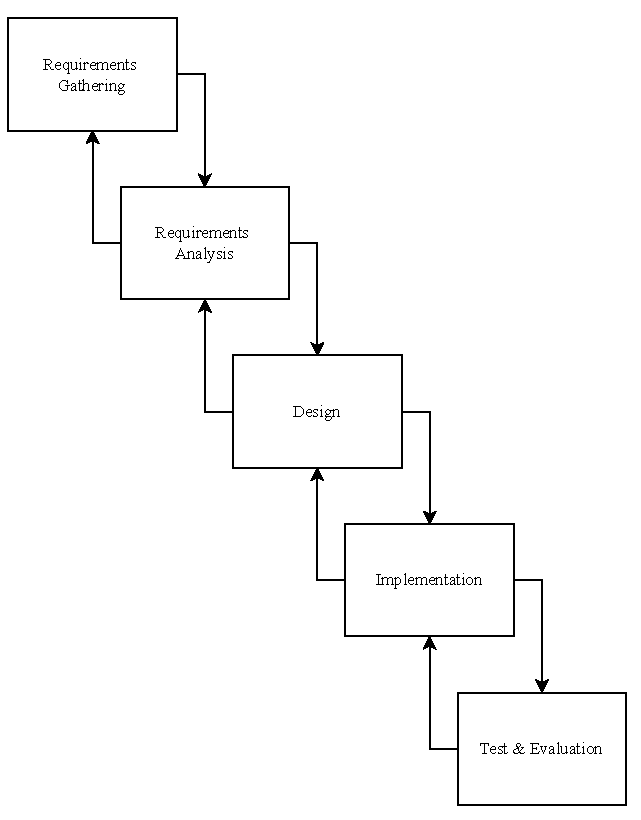
\includegraphics[width=0.7\textwidth]{figures/ResearchDesign.pdf}
	\end{figure}
	
	This study follows a modified waterfall research model to guide the development of the IoT-MCDA system shown in figure 4. The process begins with the requirements gathering, in which the system will collect comprehensive data from the Department of Agriculture (DA) and credible online datasets. The datasets include zoning information and soil parameters, as well as crop-specific requirements for growth conditions. Moreover, all datasets will be integrated with the DA’s zoning information.
	 
	It then proceeds to the requirements analysis, which identifies the need for soil health monitoring, crop prediction and fertilizer recommendation in the selected field in Region 10. A gradient boosting algorithm will be employed , using both sensor and zoning data inputs. Soil health prediction will classify soil quality levels, while crop yield forecasting will leverage an optimized machine learning model with metaheuristic-based feature selection to predict expected productivity. Fertilizer recommendations will be generated through a hybrid IoT-MCDA framework. 
	
	The next phase is the system design, where the flow of the overall system is defined with detailed descriptions on how the system will work on implementing the IoT-based ML Integration system.  This phase involves a comprehensive overview of the system design, architecture, the flowchart of the hardware and software that will be used in this system, as well as the web and mobile interfaces. The design ensures seamless integration of hardware components for data acquisition, software modules for data analysis and prediction, and user interfaces for monitoring control.
	
	This is followed by the implementation phase, which involves the development of the IoT system, training and testing of the machine learning model, in combination with multi-criteria decision analysis methods, and the configuration of hardware and software. Field nodes gather and preprocess soil data, then transmit it to a central server for storage, predictive analytics, and generation of crop suitability and fertilizer recommendations. A web dashboard visualizes soil health, farmer data, nutrient trends, weather, and zoning maps.
	
	Once completed, the testing phase is carried out in the selected area where soil data is gathered and prediction accuracy is measured. In this phase, the zoning-based recommendations are also validated. The validation phase then ensures reliability through quantitative accuracy testing and qualitative feedback on usability.  Finally, the deployment and maintenance phase presents possible large-scale applications across Region 10 with recommendations for improvement, scalability, and sustainability.

	\section{Requirements Gathering}
	The system requires comprehensive data collection to provide accurate, multi-cropping planning and fertilizer recommendation based on farming zoning in Budkinon, Philippines. Data will be sourced from the Department of Agriculture (DA), and credible online datasets. This includes detailed zoning information and soil parameters. To be included also are crop-specific requirements and growth conditions. Gathering these datasets ensures that the recommendation system is grounded in both environmental and agricultural best practices.
	 
	The types of data required encompass zoning information, and detailed crop profiles. Zoning data defines farming area, and land use classifications, while soil parameters include pH levels, matter, texture, and other essential nutrients. To be included as well is climate data such as historical rainfall, temperature, humidity, and forecast models which provide insights into environmental conditions that affect crop growth.
	
	In preparation for system integration, the data will undergo a series of preprocessing steps. Missing sensor readings and data gaps will be addressed through interpolation, while noisy or incorrect data will be identified and removed to maintain integrity. Soil and climate parameters will be normalized into uniform ranges to enhance the performance of predictive models. Once cleaned and standardized, all datasets will be integrated with the Department of Agriculture’s zoning information to ensure that recommendations are localized and relevant to the specific conditions in Bukidnon.
	
	\subsection{Research Setting}
	\begin{figure}[H]
		\centering
		\caption{System Architecture}
		\label{fig:SystemSetting}
		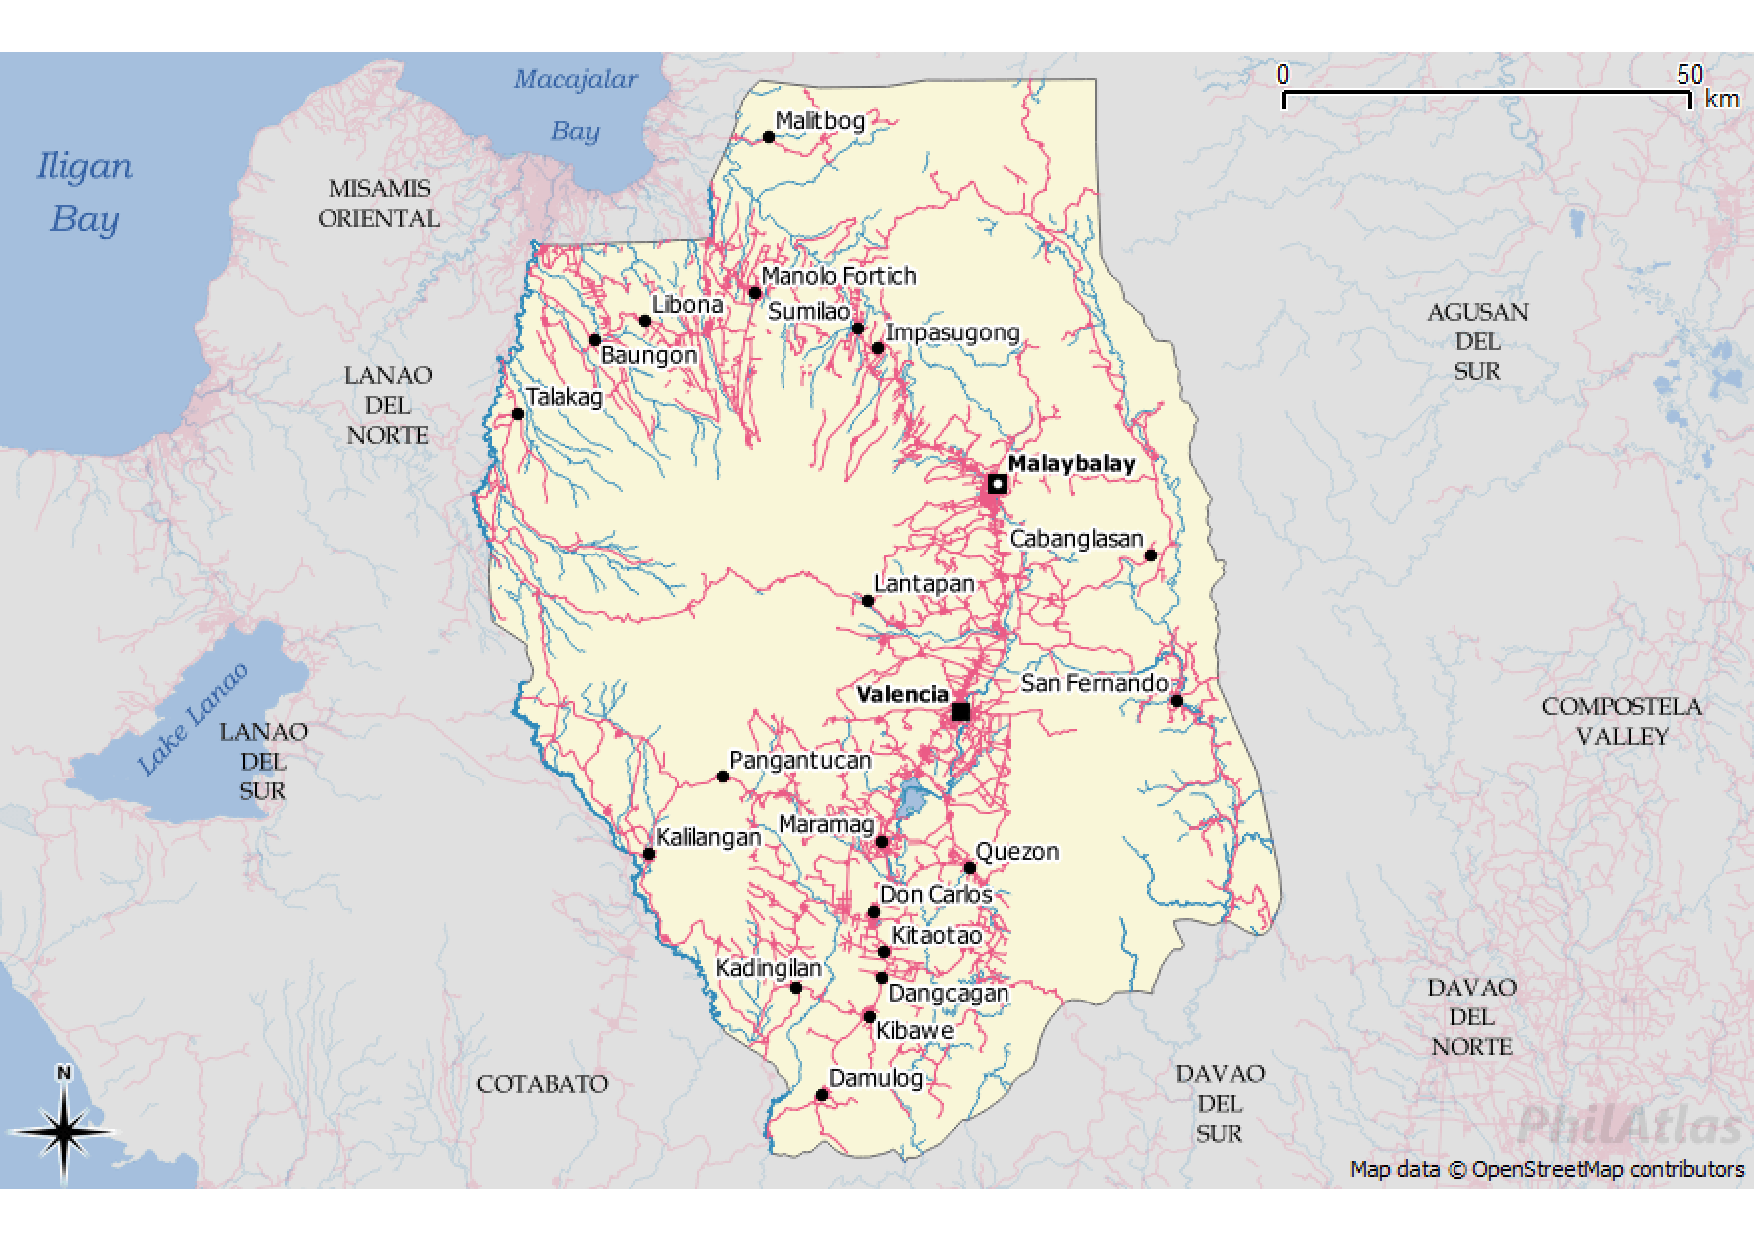
\includegraphics[width=1\textwidth]{figures/ResearchSetting.pdf}
	\end{figure}
	
	The study will be conducted on specific farms in Region 10, specifically farms in Bukidnon, Philippines. The region is mostly agricultural, with vast lands focused on the cultivation of high-value crops such as Maize (Corn), Mungbean (Mongo), Peanut, Soybean, Squash (Kalabasa), Sweet Potato (Camote), Cassava, Taro (Gabi), Eggplant, Tomato, Pechay, and Cabbage The farms in this region typically employ conventional and semi-modern farming practices, which offers a realistic setting to monitor and assess crop performance under actual farming conditions.
	
	\section{Requirements Analysis}
	The system requires the development and implementation of a machine learning component capable of performing soil health prediction, and  crop recommendation. Machine Learning boosting algorithms will be employed for these tasks, using both sensor and zoning data. Soil health prediction will classify soil quality levels, while crop yield forecasting will leverage an optimized machine learning model with metaheuristic-based feature selection to predict expected productivity. Fertilizer recommendations will be generated through a hybrid IoT-MCDA framework. Machine learning with Multi Criteria Decision Analysis will be combined to determine the most suitable fertilizer type and dosage for specific conditions. The dataset will be divided into training, validation, and testing subsets with a \texttt{70-15-15} split respectively to maximize the predictive accuracy and avoid overfitting.
	
	The system will undergo proper evaluation using both quantitative and qualitative approaches. Quantitative assessment will include metrics such as accuracy, precision, recall, and F1-score for soil health prediction. R², RMSE, and MAE for crop yield forecasting and consistency ratios and ranking stability indices for crop recommendation. Cross-validation will ensure model robustness across different crop zones. Qualitative evaluation will involve focus group discussions and structured interviews with farmers and agricultural technicians in Region 10 to assess usability, reliability, and practical value. Feedback from these sessions will guide further refinement of the system to ensure its effectiveness in real-world agricultural applications.
	
	\subsection{User Definition}
	Following the requirements analysis, the system’s users were defined as follows:
	
	\textbf{Farmer} - Farmers are the primary beneficiaries of the system. Their farms provide localized data inputs through the soil sensor. In return, farmers receive soil health insights, and multi-cropping recommendations. 
	
	\textbf{Department of Agriculture (DA)} - The DA serves as both a data provider and a supervisory user of the system. They supply zoning information, and other agricultural zoning datasets that form the foundation of the recommendation system. Through the web-based dashboard, DA officials can visualize regional soil health trends, and monitor farming zones.
	
	The specific user requirements are summarized in Table 1.
	
	\begin{table}[h!]
		\centering
		\caption{User Requirements}
		\label{tab:UserRequirements}
		\begin{tabular}{ll}
			\hline
			\textbf{User} & \textbf{Requirements} \\
			\hline
			Farmer & 
			\begin{minipage}[t]{8cm}
				- Access soil health insights (pH, moisture, nutrients) through a mobile app. \\[0.5em]
				- Receive crop suitability scores and multi-cropping recommendations. \\[0.5em]
				- Get fertilizer schedules tailored to soil condition and crop type.\\
			\end{minipage} \\
			\hline
			Department of Agriculture & 
			\begin{minipage}[t]{8cm}
				- Provide zoning maps, soil datasets, and crop profiles to the system. \\[0.5em]
				- Access a centralized web dashboard to visualize soil health, nutrient trends, and farmer data across Region 10.\\
			\end{minipage} \\
			\hline
		\end{tabular}
	\end{table}
	
	This table summarizes the requirements of the system’s two main users. Farmers need accessible insights and recommendations to guide timely crop and fertilizer decisions, while the Department of Agriculture requires integrated data and analytics to support monitoring, reporting, and regional agricultural planning. 
	
	\subsection{System Requirements}
	The system requirements shown in Table 2,  were categorized into Process, Output, Control, and Performance specifications to aid the system design and implementation.
	
	\begin{table}[h!]
		\centering
		\caption{System Requirements}
		\label{tab:SystemRequirements}
		\begin{tabular}{ll}
			\hline
			\textbf{Category} & \textbf{System Requirement} \\
			\hline
			Input Requirements & 
			\begin{minipage}[t]{8cm}
				- The system shall accept input data directly from farmers and agricultural authorities through the designated interface. \\[0.5em]
				- The system shall acquire and process soil data from integrated sensors or external data sources. \\[0.5em]
				- The system shall accept soil health data from the sensor as input for hardware operation. \\[0.5em]
				- The system shall retrieve weather information from external APIs.\\
			\end{minipage} \\
			\hline
			Process Requirements & 
			\begin{minipage}[t]{8cm}
				- The system shall combine weather, soil, and farmer-provided data into a single decision-making framework. \\[0.5em]
				- The system shall employ boosting algorithms to enhance the accuracy of predictive crop recommendations. \\[0.5em]
				- The system shall apply multi-criteria decision analysis methods to evaluate and rank potential crop options. \\[0.5em]
				
			\end{minipage} \\
			\hline
		\end{tabular}
	\end{table}
	\begin{table}[h!]
		\centering
		\begin{tabular}{ll}
			\hline
			\textbf{Category} & \textbf{System Requirement} \\
			\hline
			&
			\begin{minipage}[1]{8cm}
				- The system shall analyze data-driven insights to balance yield potential with resource availability. \\[0.5em]
				- The system shall determine an appropriate planting timeline based on environmental conditions and crop growth requirements.\\
			\end{minipage}\\
			\hline
			Output Requirements &
			\begin{minipage}[t]{8cm}
				- The system shall present crop recommendations via a visual interface on mobile and web applications. \\[0.5em]
				- The system shall display multi-cropping options, which shows compatible crop pairings. \\[0.5em]
				- The system shall present localized weather forecasts. \\[0.5em]
				- The system shall provide soil health reports with clear visual indicators.\\
				- The system shall display information on current crops cultivated by the farmer. \\[0.5em]
				- The system shall display farm details of the farmer. \\[0.5em]
				- The system shall display the locations and overview of registered farms. \\[0.5em]
				- The system shall display a list of all farmers registered. \\[0.5em]
				- The system shall present crop rules, including crop rotation guidelines, and companion planting practices.\\
			\end{minipage} \\
			\hline
			Control Requirements &
			\begin{minipage}[t]{8cm}
				- The system shall provide secure login and authentication for farmers and agricultural authorities. \\[0.5em]
			\end{minipage}\\
			\hline
		\end{tabular}
	\end{table}
	
	\begin{table} [h!]
		\centering
		\begin{tabular}{ll}
			\hline
			\textbf{Category} & \textbf{System Requirement} \\
			\hline
			&
			\begin{minipage}[t]{8cm}
				- The system shall restrict access to sensitive data based on user roles and permissions. \\[0.5em]
				- The system shall allow administrators to update crop rules and farm locations.\\
			\end{minipage} \\
			\hline				
			Performance Requirements &
			\begin{minipage}[t]{8cm}
				- The system shall scale efficiently to accommodate growth in registered farmers and farms without requiring major redesign. \\[0.5em]
				- The system must be able to have offline syncing for farmer features. \\[0.5em]					- The system must provide accurate crop recommendations for farmers.\\
			\end{minipage} \\
		\end{tabular}
	\end{table}
	
	The system requirements were defined to ensure the effective collection processing, and presentation of farm and soil data to support informed crop management decisions. The primary objective of the system is to assist farmers by integrating farm-specific information, and soil health metrics to generate accurate and actionable crop recommendations. Input requirements focus on collecting data from farmers and sensors, while process requirements involve advanced algorithms. This includes boosting algorithms, and multi-criteria-decision analysis, to evaluate and rank crop options. Outputs are delivered through mobile and web applications, to provide farmers and administrators with visualized recommendations. Control requirements ensure secure access, role-based permissions, and administrative capabilities for managing crop rules and farm records. Lastly, performance requirements address scalability, offline syncing, and recommendation accuracy, to ensure effective decision support in diverse agricultural contexts.
	
	\section{System Design}
	In this section, the flow of the overall system is defined with detailed descriptions on how the system will work on implementing the IoT-based ML integration system. This involves a comprehensive overview of the system design and architecture, and the flowchart of the hardware and software that will be used in this system. The design ensures seamless integration of hardware components for  data acquisition, software modules for data analysis and prediction, and user interfaces for monitoring and control.
	
	\subsection{System Architecture}
	\begin{figure}[H]
		\centering
		\caption{System Architecture}
		\label{fig:SystemArchitecture}
		\includegraphics[width=1\textwidth]{figures/SYSARCH.pdf}
	\end{figure}
	
	The figure \ref{fig:SystemArchitecture} illustrates the system architecture of Soil Health Monitoring, Fertilizer and Crop Recommendation for Greater Crop Yield. The system begins with a solar-powered IoT sensing unit deployed in the field. A solar panel, managed by a solar charge controller, supplies power to the entire device, ensuring continuous operation even in remote areas. The core sensing component is a soil sensor, which measures parameters such as NPK, pH, electrical conductivity, soil moisture, and temperature. Data from the sensor is transmitted through a TTL MAX485 module, which converts soil sensor signals to TTL levels readable by the ESP32 microcontroller. The ESP32 serves as the central processor, collecting sensor data, performing basic preprocessing such as averaging and sorting, attaching metadata like timestamp and location, and preparing the data for wireless transmission. For communication, the ESP32 uses a LoRa module, which allows the data to be sent over long distances to a gateway with minimal power consumption.
	
	The gateway acts as a bridge between the field device and the cloud, receiving the LoRa packets and forwarding them to the internet via Wi-Fi, Ethernet, or cellular connectivity. From there, the data is securely transmitted to Firebase, which serves as the cloud database for real-time storage and access. Once in the cloud, the raw sensor readings undergo preprocessing, validation, and enrichment with additional context such as weather or crop stage information. This cleaned data is then passed to the machine learning engine, which analyzes soil health and generates actionable outputs. Using both agronomic rules and predictive models, the system provides fertilizer recommendations, crop suggestions, and soil health scores tailored to specific field conditions.
	
	The results are delivered through two applications: the TANIM Web App and the TANIM Mobile App. The Web application is designed for agricultural authorities, providing dashboards, maps, and analytics tools to monitor soil conditions across regions and guide agricultural programs. Meanwhile, the Mobile application is aimed at farmers, offering simple and actionable insights such as soil health insights, crop recommendation and fertilizer optimization for multi-cropping. Both apps also support real-time notifications for critical issues like soil stress or device malfunctions. Importantly, farmers can provide feedback through the app, reporting crop outcomes and applied practices. This feedback, together with sensor data, is fed back into the system to retrain machine learning models and refine recommendations, creating a continuous improvement loop. Through this integration of IoT, cloud computing, and machine learning with multi-criteria decision analysis, the system enables data-driven decision-making that supports both farmers and agricultural authorities in achieving higher crop yields and sustainable farming practices.
	
	\subsection{Flowchart}
	
	\begin{figure}[H]
		\centering
		\caption{System Flowchart}
		\label{fig:SystemFlowchart}
		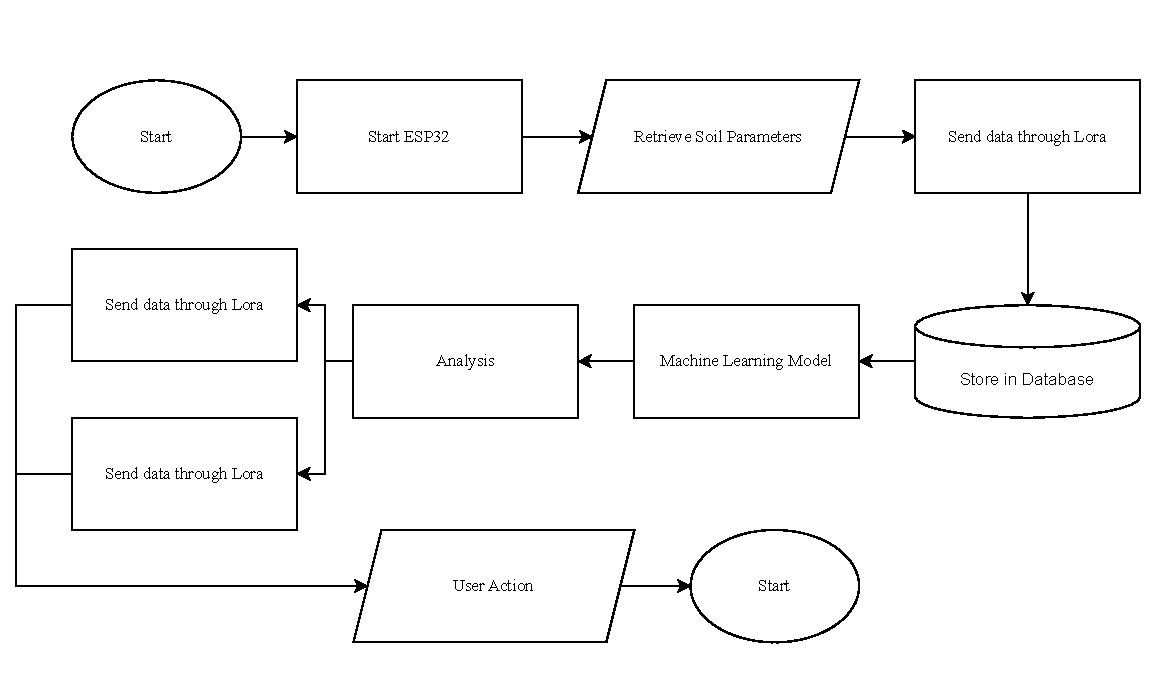
\includegraphics[width=1\textwidth]{figures/SystemFlowchart.pdf}
	\end{figure}
	
	The figure \ref{fig:SystemFlowchart} presents the operational workflow of the proposed soil health monitoring and recommendation system, highlighting the data flow from the field device to the end-user applications. The process initiates at the sensing stage, where the ESP32 microcontroller, powered through a solar energy management unit, interfaces with soil sensors to capture essential soil parameters, including Nitrogen, Phosphorus, and Potassium (NPK), pH, moisture, temperature, and soil salinity. These parameters are critical indicators of soil fertility and crop suitability. Once collected, the data is processed locally by the ESP32 to ensure efficient packaging before transmission. Leveraging LoRa technology, the device transmits the data wirelessly over long distances to a gateway, which serves as the intermediary link between the sensing unit and the cloud infrastructure. The gateway then forwards the collected data to a cloud database, ensuring reliable and scalable data storage for subsequent analysis.
	
	Within the cloud environment, the raw soil data undergoes processing and analysis through machine learning models. These models are trained on historical soil and crop datasets to identify patterns, classify soil conditions, and predict nutrient deficiencies. By transforming raw sensor readings into interpretable outputs, the system generates actionable insights regarding soil health and crop management. The analytical results include fertilizer recommendations and crop suitability assessments, enabling evidence-based decision-making for end users. This layer of intelligence ensures that data collected from the field is not merely stored but is also transformed into knowledge that directly supports precision agriculture practices.
	
	The processed insights are subsequently disseminated through two primary platforms: a web application and a mobile application. The web application is designed for agricultural authorities and extension officers, providing comprehensive monitoring dashboards, spatial analysis tools, and regional soil health reports. This enables decision-makers to track soil conditions at scale, identify priority intervention areas, and develop region-specific agricultural strategies. The mobile application targets farmers as the primary stakeholders, offering a user-friendly interface to access real-time soil health status, recommended fertilizer dosages, and crop-specific advisories. Notifications and alerts are integrated into the system to provide timely guidance, particularly in scenarios requiring immediate action.
	
	An integral component of the workflow is the feedback mechanism incorporated within both platforms. Farmers and users are able to submit observations, report crop outcomes, and validate system recommendations. This feedback not only enhances farmer engagement but also provides valuable data for iterative improvements of the machine learning models. As a result, the system establishes a continuous learning cycle wherein recommendations are refined over time, leading to greater accuracy and contextual relevance. Overall, the workflow described in Figure \ref{fig:SystemFlowchart} demonstrates how the integration of IoT sensing, cloud computing, and machine learning facilitates a comprehensive, data-driven approach to soil health management and crop productivity enhancement.
	
	\begin{figure}[H]
		\centering
		\caption{Software Mobile Application}
		\label{fig:MobileFlowchart}
		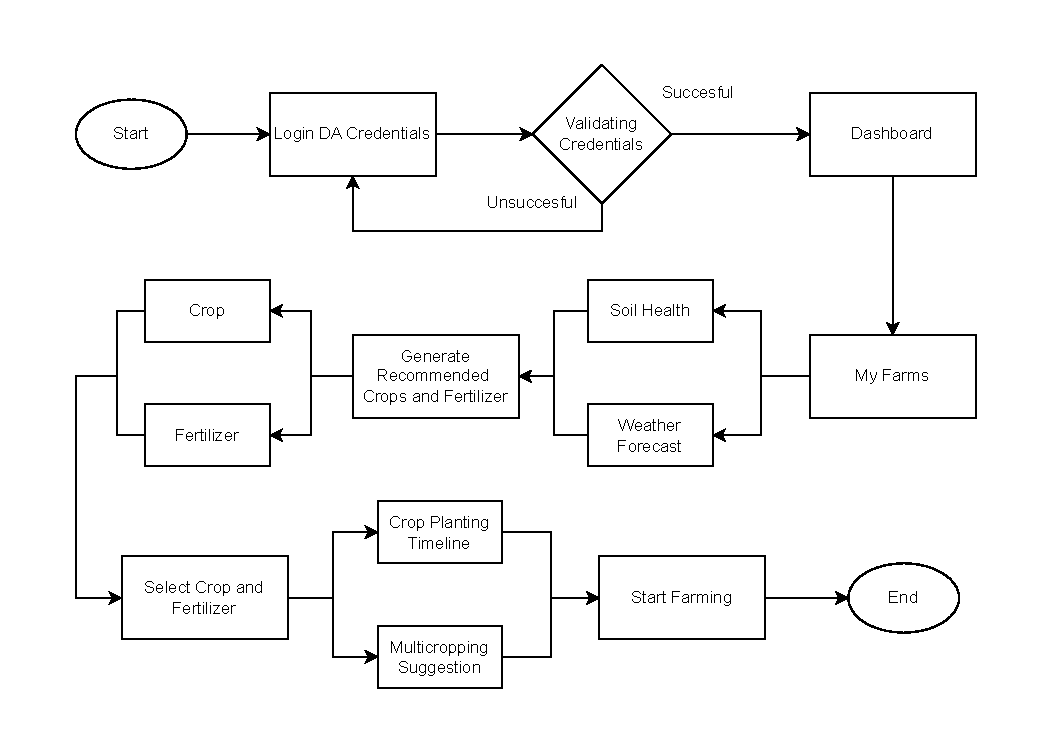
\includegraphics[width=1\textwidth]{figures/soft flow.pdf}
	\end{figure}
	
	The figure \ref{fig:MobileFlowchart} illustrates the workflow of the farming recommendation system, highlighting the interaction between farmers and the application in obtaining crop suggestions tailored to soil and weather conditions. The process begins with user authentication, wherein the farmer logs into the system using their credentials. The application validates these credentials against the stored records in the database, ensuring secure access. If the credentials are incorrect, the system prompts the user to re-enter valid information, thereby safeguarding the platform against unauthorized access. Upon successful login, the farmer is redirected to the dashboard, which serves as the central interface for accessing personalized farm data and system functionalities.
	
	From the dashboard, the farmer navigates to the “My Farms” section, where the application consolidates and displays farm-specific data. This includes soil health parameters gathered from IoT-enabled sensors and environmental information derived from integrated weather forecasting services. The system then processes this combined dataset using its analytical and decision-making algorithms to generate a list of recommended crops that are most suitable for the prevailing soil and weather conditions. By leveraging both real-time and contextual data, the system ensures that the recommendations are accurate, adaptive, and relevant to the farmer’s specific location and situation. Once the recommendations are presented, the farmer can review the options and select the crop that aligns with their goals, preferences, and available resources. Following this selection, the system provides advanced features designed to further support farm management. These include multicrop suggestions, which propose crop diversification strategies for risk mitigation and sustainable land use, as well as a detailed crop planting timeline that outlines optimal planting and cultivation schedules. Such features are aimed at enhancing farming efficiency, improving resource allocation, and maximizing yield potential.
	
	The final stage of the workflow involves the farmer applying the recommendations provided by the system. By combining data-driven crop selection with structured guidance on crop management, the system enables farmers to initiate the farming process with greater confidence and scientific support. This workflow underscores the system’s capacity to guide users from initial login and farm data access to informed decision-making and implementation in the field. Ultimately, the integration of secure user access, real-time soil and weather data, intelligent recommendation algorithms, and decision support tools demonstrates how the farming recommendation system contributes to improved agricultural productivity and long-term sustainability.
	
	\begin{figure}[H]
		\centering
		\caption{Web Application Flowchart}
		\label{fig:WebFlowchart}
		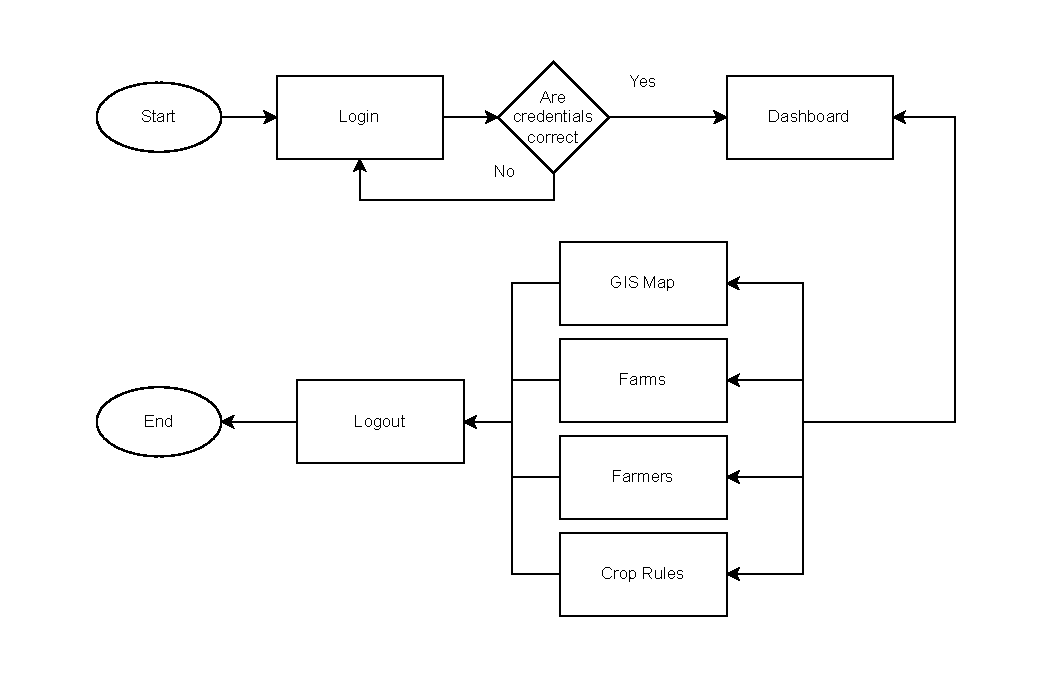
\includegraphics[width=1\textwidth]{figures/web flow.pdf}
	\end{figure}
	
	Figure \ref{fig:WebFlowchart} illustrates the workflow of the Farm Management Web Application, which is specifically designed to support agriculture administrators in managing and monitoring farming activities at a broader scale. The process begins with a secure login mechanism, wherein the administrator is required to enter valid credentials. The system validates these credentials against stored records to ensure authorized access. If the login attempt is unsuccessful, the administrator is prompted to re-enter the correct credentials, thereby maintaining both system integrity and data security. Once authenticated, the administrator is directed to the main dashboard, which functions as the central control panel for the application.
	
	From the dashboard, administrators are provided with access to several key modules, each serving a distinct role in farm management. The Farms module enables the management of farm records, including details such as farm size, location, and soil health data. The GIS Map module provides geospatial visualization, allowing administrators to monitor farm distribution, analyze spatial patterns, and make data-driven decisions at the regional level. The Farmers module consolidates and manages farmer profiles, enabling oversight of farmer registration, activity logs, and engagement with advisory services. The Crop Rules module supports the definition, modification, and enforcement of agricultural guidelines, such as fertilizer application standards, crop suitability rules, and sustainability practices. These modules are seamlessly integrated with the dashboard, ensuring smooth navigation and centralized administration. 
	
	Additionally, the system provides administrators with the option to securely terminate their session at any point through the logout function, further reinforcing data protection and privacy. By integrating secure access control with comprehensive management modules, the Farm Management Web Application ensures that administrators maintain full oversight of agricultural data, farmer engagement, and policy implementation. This workflow demonstrates how the system empowers administrators to efficiently coordinate farm-level operations while supporting evidence-based decision-making, regional monitoring, and sustainable agricultural governance.
	
	\subsection{Context Level Diagram}
	The Context-Level Diagram provides a high-level view of how the TANIM system interacts with its primary stakeholders: Agricultural Authorities and Farmers. It illustrates how data flows into and out of the system without detailing internal processes.
	
	\begin{figure}[H]
		\centering
		\caption{Context-Level Diagram Between the System And Agricultural Authorities}
		\label{fig:CLDSystem&AgriAuthorities}
		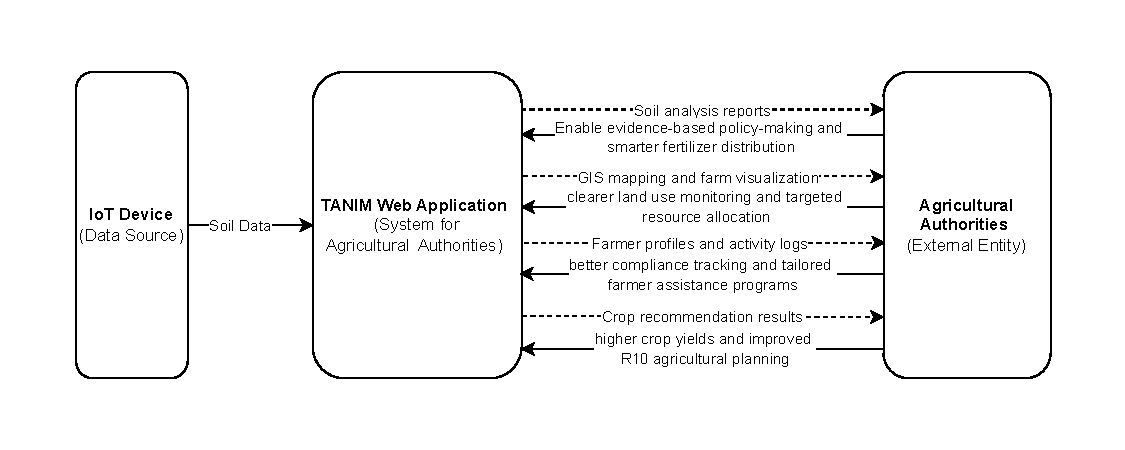
\includegraphics[width=1\textwidth]{figures/cldWEB.pdf}
	\end{figure}
	
	The Figure \ref{fig:CLDSystem&AgriAuthorities} presents the interaction between Agricultural Authorities and the TANIM Web 	Application from the perspective of informational input and decision-making output. While authorities do not directly generate the raw data, they receive processed insights derived from IoT devices deployed in the field. These insights include soil analysis reports, GIS-based farm visualization, farmer profiles, and crop recommendation results. Each of these outputs enables corresponding benefits such as evidence-based policy-making, targeted resource allocation, compliance tracking, and improved agricultural planning. In this way, TANIM translates raw field data into actionable intelligence, empowering authorities to make informed, timely, and sustainable decisions that support both farmers and national food security goals.
	
	\begin{figure}[H]
		\centering
		\caption{Context-Level Diagram Between the System And Farmers}
		\label{fig:CLDSystem&Farmers}
		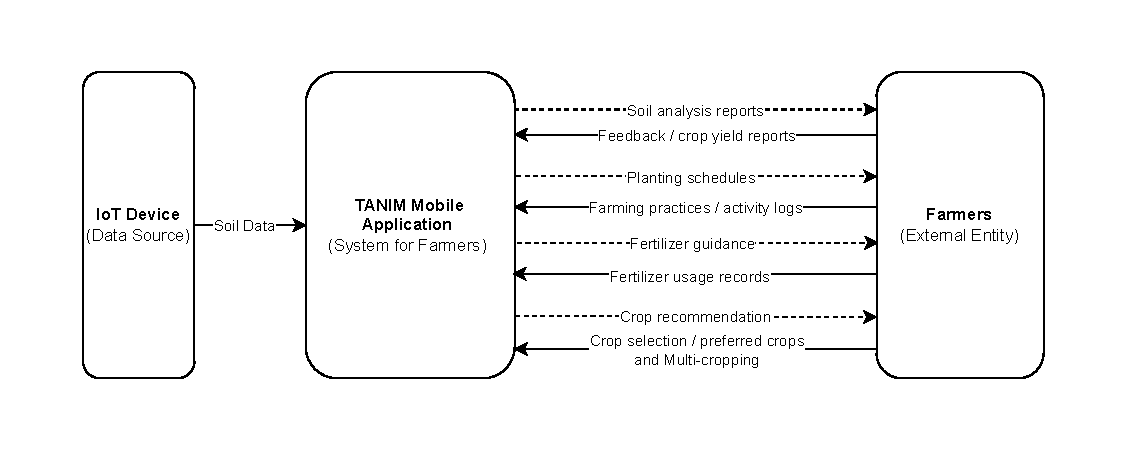
\includegraphics[width=1\textwidth]{figures/cldMOB.pdf}
	\end{figure}
	
	The figure \ref{fig:CLDSystem&Farmers} illustrates the interaction of the TANIM Mobile Application with farmers and IoT devices. IoT devices act as data sources, providing soil and environmental information to the system, which then processes the data to deliver outputs such as soil analysis reports, planting schedules, fertilizer guidance, crop recommendations, and farming practice records. Farmers, as external entities, contribute by supplying inputs like crop yield feedback, farming activity logs, fertilizer usage records, and crop preferences. This exchange of data ensures that the system can generate accurate recommendations, supporting sustainable farming practices and helping farmers improve productivity and decision-making
	
	\subsection{Data Flow Diagram}
	The Data Flow Diagram visually represents how data flows within the TANIM system. It highlights the interactions between IoT devices, farmers/agricultural authorities, and the system’s core processes, demonstrating how data is retrieved, stored, and analyzed to provide soil health insights and crop/fertilizer recommendations.
	
	\begin{figure}[H]
		\centering
		\caption{Data Flow Diagram}
		\label{fig:DFD}
		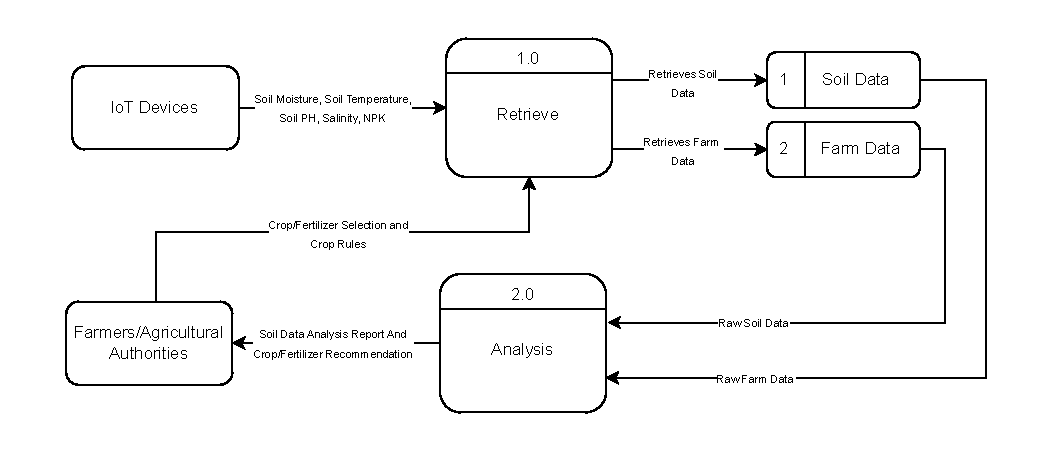
\includegraphics[width=1\textwidth]{figures/DFD.pdf}
	\end{figure}
	
	Figure \ref{fig:DFD} shows the Data Flow Diagram (DFD) of the TANIM system. The data flow between the user and the system is divided into two main processes: retrieval and analysis. The “retrieve” process is responsible for collecting soil and farm data from IoT devices, as well as crop and fertilizer inputs from the users. These data are then stored in the system’s database for access and processing. The “analysis” process uses the stored data to assess soil health conditions and generate crop or fertilizer recommendations. Finally, the processed results are delivered to farmers or agricultural authorities in the form of soil data analysis reports and practical recommendations to support better agricultural decision-making.
	
	\subsection{Use Case Diagram}
	The Use Case Diagram visually represents how different actors interact with the system of TANIM. It illustrates both passive and active engagements that facilitate data collection and system utilization.
	
	\begin{figure}[H]
		\centering
		\caption{Farmer Use Case Diagram}
		\label{fig:FarmerUseCase}
		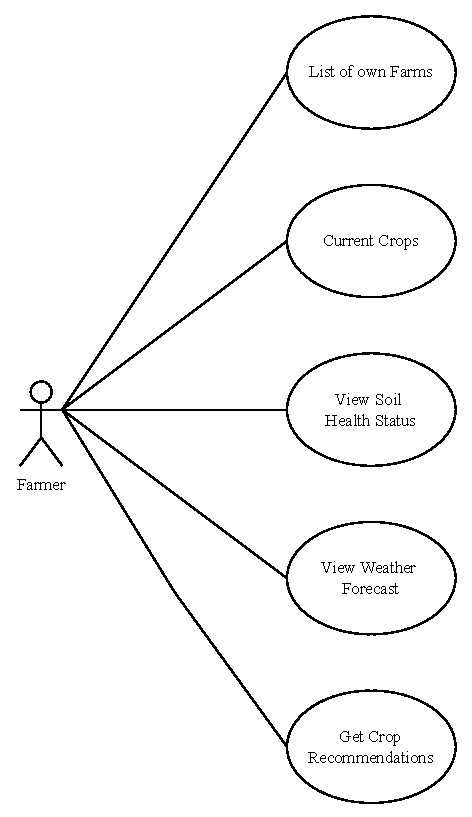
\includegraphics[width=0.5\textwidth]{figures/FarmerUseCase.pdf}
	\end{figure}
	
	Figure \ref{fig:FarmerUseCase} shows how Farmers interact with the system. Farmers can use the system to view a list of their own farms, which helps them keep track of their agricultural activities in an organized manner. They are also able to check the status of their crops in the corresponding farm. This allows them to stay updated on growth progress and overall crop status. In addition, the system enables farmers to monitor soil health, Farmers can also access weather updates directly through the platform, which is essential for planning day-to-day tasks and preparing for potential challenges. Lastly, the system provides personalized crop recommendations, giving farmers guidance that is tailored to their specific conditions and needs. Together, these features create a comprehensive tool that supports farmers in managing their farms more effectively.
	
	\begin{figure}[H]
		\centering
		\caption{Use Case Diagram of Department of Agriculture}
		\label{fig:DAUseCase}
		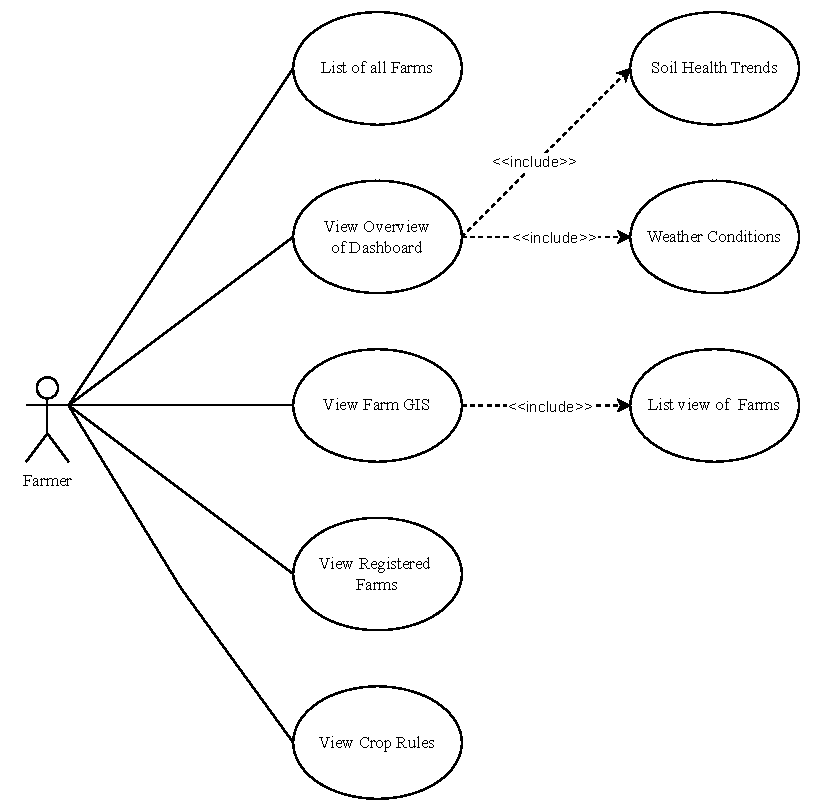
\includegraphics[width=1\textwidth]{figures/DAUseCase.pdf}
	\end{figure}
	
	Figure \ref{fig:DAUseCase} shows how the Department of Agriculture interacts with the system. The Department of Agriculture can access everything the farmer has access to, in addition, the Department of Agriculture can utilize a comprehensive dashboard that provides weather insights, which gives a clear overview of conditions that may affect multiple farms at once.  It also has the ability to manage all farm listings. Another important function is the use of GIS maps to view farm locations, allowing for a view of agricultural activity across different areas. Lastly, the Department can oversee crop-related regulations, ensuring that standards are properly implemented.
	
	\subsection{Hardware Design Flowchart}
	\begin{figure}[H]
		\centering
		\caption{Hardware Design Flowchart}
		\label{fig:HardwareFlowchart}
		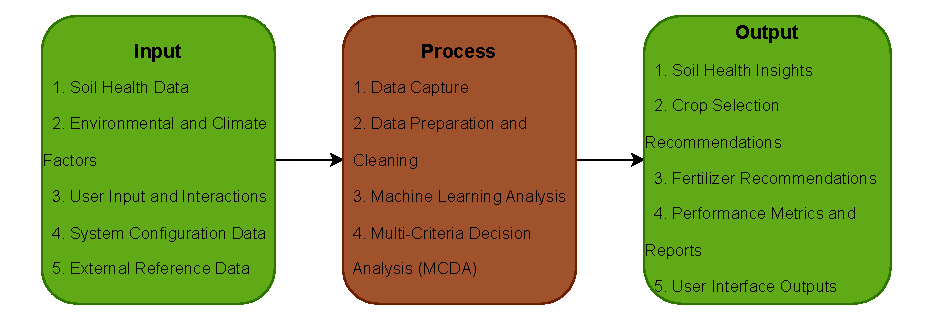
\includegraphics[width=1\textwidth]{figures/IPO.pdf}
	\end{figure}
	
	Figure \ref{fig:HardwareFlowchart} illustrates the workflow of the hardware components. Figure 15 illustrates the workflow of the hardware components. The process begins at the "Start" node, followed by the initialization of the central microcontroller. Next, the sensor is initialized to prepare for data collection. Once the sensor retrieves data, the process moves to the transceiver module, which handles the transmission of the collected data. The transmitter module then processes and sends the data, concluding the workflow at the "End" node.
	
	The flowchart represents a sequential hardware operation where each step is dependent on the successful completion of the previous one. The microcontroller acts as the brain, controlling the sensor initialization and data retrieval. The transceiver module facilitates communication, while the transmitter module ensures the data is sent effectively, completing the hardware cycle.
	
	\subsection{3D Design}
	\begin{figure}[H]
		\centering
		\caption{3D Container Design}
		\label{fig:3D}
		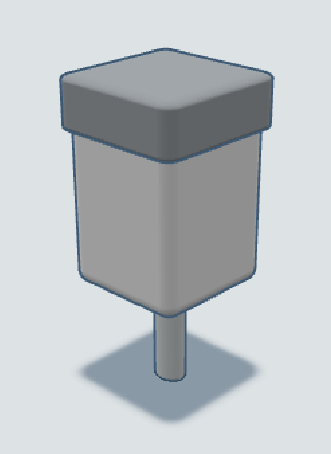
\includegraphics[width=0.5\textwidth]{figures/3D.pdf}
	\end{figure}
	
	Figure \ref{fig:3D} displays the 3D container design that will be 3D printed for the container of the hardware. This will contain the hardware components which are etched in a PCB board that will be used in this system. The container should be durable to ensure that it can secure the hardware components inside of it.
	
	\subsection{Materials and Cost}
	\begin{table}[h!]
		\centering
		\caption{Hardware Components and Cost}
		\label{tab:MaterialsAndCost}
		\begin{tabular}{ll}
			\toprule
			\textbf{Component} & \textbf{Price} \\ 
			\midrule
			Microprocessor & \textpeso 150 \\ 
			\hline
			Soil Sensor & \textpeso 1,654.90 \\
			\hline
			Solar Power Manager & \textpeso 860 \\
			\hline
			Solar Panel & \textpeso 320 \\
			\hline
			Lithium Ion Battery & \textpeso 120 \\
			\hline
			Transceiver Module & \textpeso 163 \\
			\hline
			Transmitter Module & \textpeso 180 \\
			\hline
			Miscellaneous (Cable, Mounts) & \textpeso 1,500 \\
			\textbf{Total} & \textbf{\textpeso 4,947.90} \\
			\bottomrule
		\end{tabular}
	\end{table}
	
	\section{Implementation}
	The Implementation phase involves developing the software and hardware components. Each function was ensured to function according to the design specifications.This phase intends to transform the conceptual design into a working prototype that can perform data acquisition, processing, and output for TANIM.
	
	\subsection{Software Implementation}
	The software implementation for TANIM is designed to provide an efficient, reliable, and user-friendly platform that caters to the needs of both the Farmer and The Department of Agriculture. To ensure optimal accessibility and performance, the frontend for farmers is developed using React Native, a framework well-suited for creating responsive mobile applications. While the frontend for the Department of Agriculture is implemented using React.js, which allows for seamless web application experience. Both user interfaces interact with a shared backend developed in Flask, which centralizes data management and ensures consistent functionality across platforms. This architecture aids in efficient communication between the mobile and web applications. It also supports scalability, and maintainability and ease of integration with additional features or services in the future.
	
	\subsection{Hardware Implementation}
	The hardware implementation of the TANIM system is centered on an IoT-based device designed to collect soil data and send it to the cloud for processing and analysis. The core of the device is an ESP32 microcontroller, due to its high processing capability, built-in Wi-Fi, and compatibility with multiple sensor modules.  A soil sensor is used to monitor key soil parameters such as NPK, moisture, temperature, and pH. Meanwhile a TTL MAX485 module facilitates reliable communication between the sensors and the ESP32. Data transmission is handled via a LoRa module, which provides long-range, and low-power communication to a central gateway. The system is to be powered by a solar panel managed through a dedicated solar panel manager. The modular design of the hardware makes the system scalable and adaptable to changing agricultural environments.
	
	\subsection{Data Acquisition and Storage}
	The sensor is tasked with acquiring data by measuring a variety of critical indicators of soil health. The collected data is then sent to a cloud storage, which provides a secure, scalable, and easily accessible repository for large volumes of environmental data. This cloud-based storage solution not only ensures data integrity and reliability but also facilitates seamless integration with processing stages. The stored data is then utilized as input for the trained machine learning model, which analyzes the information to generate precise insights, predictions, and recommendations regarding soil conditions. Overall, this supports informed decision-making for agricultural management.
	
	\subsection{Machine Learning Model}
	The TANIM system will use a boosting algorithm as the core of its predictive model, chosen for its efficiency, scalability, and high accuracy in handling large and complex datasets. This machine learning approach is combined with Multi-Criteria Decision Analysis (MCDA) methods, to provide crop recommendations that consider multiple factors such as soil type, weather conditions, and historical yield data. By integrating machine learning boosting algorithms and Multi-Criteria Decision Analysis, the system is able to deliver personalized and data-driven crop recommendations that optimize productivity and efficient crop utilization.
	
	\section{Test and Evaluation}
	Testing and evaluation will be conducted to verify the system’s effectiveness, accuracy, and usability for crop recommendation and soil health monitoring. This process will be designed to ensure that the hardware components, software components, and machine learning models will function according to what we aim for this study, which involves hardware testing and calibration, functional testing, system integration testing, performance testing, and usability testing. Hardware testing and calibration will focus on verifying the accuracy of the sensors to ensure reliable soil data. Functional testing will examine whether the mobile and web applications operate correctly and deliver the expected outputs of each feature. To ensure that the hardware, cloud database, machine learning, and applications works together with proper data flow and error handling, system integration will be implemented. For measuring the responsiveness of the system and to evaluate the system’s predictive accuracy of the machine learning models using various performance metrics we will be conducting performance testing. Moreover, usability testing will assess the practicality and user-friendliness of the system by involving farmers and agricultural experts in field trial and feedback collection.
	
	\subsection{Hardware Testing and Calibration}
	Hardware testing and calibration will ensure that the IoT sensors will provide accurate measurements of soil health parameters such as nitrogen, phosphorus, potassium, pH, moisture, salinity, and temperature. To conduct this testing, the sensors will be deployed in field testing on the actual farms in Region 10, also to ensure consistency under varying field conditions the readings will be recorded at different time and day. Cross checking will be applied by using the Department of Agriculture’s soil testing laboratory and soil test kits of the same soil samples from the same farms to ensure reliability and accuracy.
	
	Through statistical measures such as Mean Absolute Error (MAE) the sensor readings will be compared against laboratory results. a maximum allowable error threshold of ±5 will be set, if the difference between the sensor and laboratory values exceeds this threshold error, calibration adjustments will be applied to the sensors until acceptable accuracy will be achieved. It will be calculated by:
	
	
	\textbf{EQUATION DIRI}
	
	This process ensures that the data generated by the hardware is reliable enough to be used in machine learning models and the recommendation system.
	
	\subsection{Functional Testing}
	Functional testing involves verifying whether each feature of the mobile and web applications operates correctly according to the system design. For the mobile application, the following features will be tested: secure login and authentication, retrieval of soil health readings, display of crop recommendation for multi-cropping, fertilizer optimization, and offline data synchronization. For the web application, features like farm visualization, farmer profile management, and crop rules will be tested.
	
	Each feature will be executed under controlled test cases and the outcomes will be analyzed against the desired output. Additionally, stress tests will be conducted by simulating multiple user logins and farm entries simultaneously to evaluate the application performance. Through this process it ensures that the mobile and web applications behave correctly as intended and is reliable for real-world scenarios of farmers and agricultural authorities.
	
	\subsection{System Integration Testing}
	System integration testing will evaluate whether the hardware, software, cloud database, and machine learning model communicates seamlessly with each other as a single system. The system integration testing will be tested by following the full flow of the system: soil health readings captured by the sensor and processed by the ESP32 microcontroller, then transmitted by via the LoRa module to the gateway, forwarded to the cloud database, then processed by the machine learning models, and finally displayed on the mobile and web applications. 
	
	This process confirms that the system works together as one reliable system. Furthermore, tests will be conducted to observe how the system handles incomplete or corrupted data to ensure that it can manage error to prevent misleading recommendations to farmers.
	
	\subsection{Performance Testing}
	For the system level performance, it is to determine if the system could handle multiple data acquisition and provide timely feedback to the users. The data transmission success rate will be monitored by comparing the successful sensor to cloud uploads against the attempted uploads over multiple trials. Latency tests measure the time from the sensor data capture to its display in the mobile and web application, with an acceptable range set to 30 seconds. Scalability will be evaluated by simulating multiple farms connected simultaneously to ensure that the cloud database and applications could handle increased workloads without delays and crashes. These will ensure that the system is reliable and efficient under real-world agricultural conditions where multiple users operate.
	
	For the machine learning evaluation, it verifies the predictive capability of the machine learning models that will be used on crop recommendation for multi-cropping and fertilizer optimization. The dataset will be split into 70-15-15 for training, evaluation, and testing for maximizing the predictive accuracy and avoiding overfitting. 
	
	For the crop recommendation, the machine learning models will be evaluated using accuracy, precision, recall, F1-score, and confusion matrices to determine the effectiveness of the system. The following formulas are going to be use:
	
	\textbf{TANAN FORMULA}
	
	The Multi-Criteria Decision Analysis (MCDA) process will be tested by computing the Analytic Hierarchy Process (AHP) consistency ratio, which was required to be less than 0.1 for validity, and by checking the stability of crop rankings produced through TOPSIS. These evaluation steps confirm that the machine learning models not only provide scientifically sound predictions but also deliver recommendations that are consistent and stable under different scenarios.
	
	\subsection{Usability Testing}
	The usability testing will assess the practicality, accessibility, and user satisfaction of the system. For this, farmers will be asked to log into the mobile application, review soil health data, view crop and fertilizer recommendations, and simulate updating their farm records. Meanwhile, DA officials will use the web dashboard to access farmer profiles, view GIS-based maps, and manage crop rules.
	
	After completing the navigation of the system, the System Usability Scale (SUS) developed by Brooke (1995) will be employed. The interactions of the users will be observed and the difficulties they encountered will be recorded. Also, feedback will be collected to gain insights into what features were most useful, and which feature needs improvement. This testing ensures that the system will be accessible, user-friendly, and is beneficial to the users.
	
}
